\documentclass[10pt,landscape]{article}
\usepackage{multicol}
\usepackage{calc}
\usepackage{ifthen}
\usepackage[landscape]{geometry}
\usepackage{graphicx}
\usepackage{amsmath, amssymb, amsthm}
\usepackage{latexsym, marvosym}
\usepackage{pifont}
\usepackage{lscape}
\usepackage{graphicx}
\usepackage{array}
\usepackage{booktabs}
\usepackage[bottom]{footmisc}
\usepackage{tikz}
\usetikzlibrary{shapes}
\usepackage{pdfpages}
\usepackage{wrapfig}
\usepackage{enumitem}
\setlist[description]{leftmargin=0pt}
\usepackage{xfrac}
\usepackage[scr=boondoxo,scrscaled=1.05]{mathalfa}
\usepackage[pdftex,
            pdfauthor={Kevin Hartman},
            pdftitle={W203 Unit Summary},
            pdfsubject={A pdf and reference guide for MIDS W203, Probability and Statistics for Data Science.},
            pdfkeywords={probability} {statistics} {guide} {pdf} {reference} {sheet} {formulas} {equations}
            ]{hyperref}
\usepackage[
            open,
            openlevel=2
            ]{bookmark}
\usepackage{relsize}
\usepackage{rotating}
\usepackage{bbm}

\newcommand\independent{\protect\mathpalette{\protect\independenT}{\perp}}
  \def\independenT#1#2{\mathrel{\setbox0\hbox{$#1#2$}%
  \copy0\kern-\wd0\mkern4mu\box0}} 
    
\newcommand{\noin}{\noindent}    
\newcommand{\logit}{\textrm{logit}} 
\newcommand{\var}{\textrm{Var}}
\newcommand{\cov}{\textrm{Cov}} 
\newcommand{\corr}{\textrm{Corr}} 
\newcommand{\N}{\mathcal{N}}
\newcommand{\Bern}{\textrm{Bern}}
\newcommand{\Bin}{\textrm{Bin}}
\newcommand{\Beta}{\textrm{Beta}}
\newcommand{\Gam}{\textrm{Gamma}}
\newcommand{\Expo}{\textrm{Expo}}
\newcommand{\Pois}{\textrm{Pois}}
\newcommand{\Unif}{\textrm{Unif}}
\newcommand{\Geom}{\textrm{Geom}}
\newcommand{\NBin}{\textrm{NBin}}
\newcommand{\Hypergeometric}{\textrm{HGeom}}
\newcommand{\HGeom}{\textrm{HGeom}}
\newcommand{\Mult}{\textrm{Mult}}

    
%\newenvironment{proof}[1][Proof]{\begin{trivlist}
%\item[\hskip \labelsep {\bfseries #1}]}{\end{trivlist}}
\newenvironment{definition}[1][Definition]{\begin{trivlist}
\item[\hskip \labelsep {\bfseries #1}]}{\end{trivlist}}
\newenvironment{example}[1][Example]{\begin{trivlist}
\item[\hskip \labelsep {\bfseries #1}]}{\end{trivlist}}
\newenvironment{remark}[1][Remark]{\begin{trivlist}
\item[\hskip \labelsep {\bfseries #1}]}{\end{trivlist}}

% To make this come out properly in landscape mode, do one of the following
% 1.
%  pdflatex Statisticscheat.tex
%
% 2.
%  latex Statisticscheat.tex
%  dvips -P pdf  -t landscape Statisticscheat.dvi
%  ps2pdf Statisticscheat.ps

% This sets page margins to .5 inch if using letter paper, and to 1cm
% if using A4 paper. (This probably isn't strictly necessary.)
% If using another size paper, use default 1cm margins.
\ifthenelse{\lengthtest { \paperwidth = 11in}}
	{ \geometry{top=.4in,left=.2in,right=.2in,bottom=.4in} }
	{\ifthenelse{ \lengthtest{ \paperwidth = 297mm}}
		{\geometry{top=1cm,left=1cm,right=1cm,bottom=1cm} }
		{\geometry{top=1cm,left=1cm,right=1cm,bottom=1cm} }
	}

% Turn off header and footer
\pagestyle{empty}
 

% Redefine section commands to use less space
\makeatletter
\renewcommand{\section}{\@startsection{section}{1}{0mm}%
                                {-1ex plus -.5ex minus -.2ex}%
                                {0.5ex plus .2ex}%x
                                {\normalfont\large\bfseries}}
\renewcommand{\subsection}{\@startsection{subsection}{2}{0mm}%
                                {-1explus -.5ex minus -.2ex}%
                                {0.5ex plus .2ex}%
                                {\normalfont\normalsize\bfseries}}
\renewcommand{\subsubsection}{\@startsection{subsubsection}{3}{0mm}%
                                {-1ex plus -.5ex minus -.2ex}%
                                {1ex plus .2ex}%
                                {\normalfont\small\bfseries}}
\makeatother

% Define BibTeX command
\def\BibTeX{{\rm B\kern-.05em{\sc i\kern-.025em b}\kern-.08em
    T\kern-.1667em\lower.7ex\hbox{E}\kern-.125emX}}

% Don't print section numbers
\setcounter{secnumdepth}{0}


\setlength{\parindent}{0pt}
\setlength{\parskip}{0pt plus 0.5ex}


% -----------------------------------------------------------------------

\usepackage{titlesec}

%\titleformat{\section}
%{\color{blue}\normalfont\large\bfseries}
%{\color{blue}\thesection}{1em}{}
%\titleformat{\subsection}
%{\color{cyan}\normalfont\normalsize\bfseries}
%{\color{cyan}\thesection}{1em}{}
% Comment out the above 5 lines for black and white

\usepackage{Sweave}
\begin{document}
\Sconcordance{concordance:W203_Unit_Summary.tex:W203_Unit_Summary.Rnw:%
1 132 1 1 0 408 1 1 10 6 1 1 10 268 1}



\raggedright
\footnotesize
\begin{multicols}{3}


% multicol parameters
% These lengths are set only within the two main columns
%\setlength{\columnseprule}{0.25pt}
\setlength{\premulticols}{1pt}
\setlength{\postmulticols}{1pt}
\setlength{\multicolsep}{1pt}
\setlength{\columnsep}{2pt}

\begin{center}
     \Large{\textbf{W203 Unit Summary}} \\
\end{center}

\scriptsize

%Compiled from notes taken by Kevin Hartman (\url{http://kevin-hartman.github.io}), with additional material and template format taken from the Probability Cheatsheet v2.0 by William Chen (\url{http://wzchen.com}), Joe Blitzstein, Sebastian Chiu, Yuan Jiang, Yuqi Hou, and Jessy Hwang. Licensed under \texttt{\href{http://creativecommons.org/licenses/by-nc-sa/4.0/}{CC BY-NC-SA 4.0}}.

%%%%%%%%%%%%%%%%%%%%%%%%%%%%%%%%%%%%%%%%%%%%%%%%%%%%%%%%%%%%%%%%
% Unit 1: Descriptive Statistics
%%%%%%%%%%%%%%%%%%%%%%%%%%%%%%%%%%%%%%%%%%%%%%%%%%%%%%%%%%%%%%%%
\section{Unit 1. Descriptive Statistics}
	\subsection{Terms and Definitions}
\begin{description}
\item[Population:] a well-defined collection of objects in an area of interest (investigation)
\item[Census:] an occurance of availability of desired information for all objects in the population
\item[Sample:] a subset of the population, selected in some prescribed manner
\item[Characteristic:] an attribute of the data, which may be categorical or numerical
\item[Variable:] any characteristic whose value may change from one object to another in the population
\item[Univariate:] a data set that consists of observations on a single variable
\item[Multivariate:] a data set that consists of observations on multiple variables
\item[Bivariate:] a data set that consists of observations on two variables specifically
\item[Descriptive Statistics:] the branch of statistics that summarizes and describes important features of the data
\item[Inferential Statistics:] the branch of statistics that draws a form of conclusion about the population from the sample
\item[Probability:] the bridge between descriptive and inferential techniques. In probability, properties of the population are assumed known, and questions are posed and answered from a representative sample.
\item[Discrete and Continuous Variables:] A numerical variable is $discrete$ if its set of possible values is at most countable. A numerical value is $continuous$ if its set of possible values is an uncountable set.\\

Probability: population $\to$ sample\\
Stats: sample $\to$ population\\
\end{description}
\subsection{Measures of Location}
For observations $x_1, x_2, \cdots, x_n$
\begin{description}
	\item[Sample Mean:] $\bar{x} = \frac{\sum_{1=1}^{n} x_i}{n}$
	\item[Sample Median:] $\tilde{x} = \left\{\begin{array}{lr} \left(\frac{n+1}{2} \right)^{th} \text{if n is odd} \\ \text{avg of } \left(\frac{n}{2}\right)^{th} \text{\&} \left(\frac{n}{2} + 1\right)^{th} \text{if n is even} \end{array} \right.$
	\item[Trimmed Mean:]	a compromise between $\tilde x$ and $\bar{x}$ by removing a percentage of the smallest and largest observations
\end{description}

\subsection{Measures of Variability}
\begin{description}
	\item[Range:] the difference betwen the largest and smallest sample variables
	\item[Sample Variance:] $\sigma^2 = \frac{S_{xx}}{n-1}=\frac{\sum_{i=1}^n(x_i-\bar{x})^2}{n-1}$
	\item[Sample Standard Deviation:] $\sigma = \sqrt{\sigma^2}$
	\item[Properties:] Let $x_1, x_2, \dots, x_n$ be a sample and $c$ be any nonzero constant.\\
1. If $y_1 = x_1 + c, y_2 = x_2 + c,\dots, y_n = x_n + c$, then $\sigma_y^2 = \sigma_x^2$ and \\
2. If $y_1 = cx_1,\dots,y_n=cx_n$, then $\sigma_y^2=c^2s_x^2$, $\sigma_y=|c|s_x$\\
where $\sigma_x^2$ is the sample variance of the $x$'s and $\sigma_y^2$ is the sample variance of the $y$'s.\\
\end{description}

\subsection{Box Plots}
\begin{description}
  \item[Upper Fourth:] the median of the largest half of observations
  \item[Lower Fourth:] the median of the smallest half of observations
  \item[Fourth Spread:] $f_s$ = upper fourth - lower fourth
  \item[Outlier:] any observation farther than $1.5f_s$ from the closest fourth (considered mild if less than $3f_s$)
  \item [Extreme Outlier:] an observation farther than $3f_s$ from the nearest fourth
  \item[Sample Covariance:] The simplest measure of association between two variables. $$cov(x,y)=\frac{\sum_{i=1}^n(x_i-\bar{x})(y_1-\bar{y})}{n-1}$$
  \item[Sample Correlation:] Measures the linear relationship between two variables. $$r_{x,y}=\frac{cov(x,y)}{s_xs_y}$$
  \item[Properties:] \quad \\
1. Adding $c$ to variable $x$ or variable $y$ doesn't change $r_{x,y}$\\
2. Multipling a non-zero $c$ to variable $x$ or variable $y$ doesn't change $r_{x,y}$
\end{description}

%%%%%%%%%%%%%%%%%%%%%%%%%%%%%%%%%%%%%%%%%%%%%%%%%%%%%%%%%%%%%%%%
% Unit 3: Probability Theory
%%%%%%%%%%%%%%%%%%%%%%%%%%%%%%%%%%%%%%%%%%%%%%%%%%%%%%%%%%%%%%%%
\section{Unit 3. Probability Theory}
	\subsection{Terms and Definitions}
\begin{description}
	\item[Experiment:] any activity or process whose outcome is subject to uncertainty
	\item[Sample Space:] denoted by $\mathscr{S}$, is the set of all possible outcomes of an experiment
	\item[Event Space:] denoted by $\mathscr{F}$, is the subset of outcomes from the sample space. It includes  subsets of $\mathscr{S}$, the empty set $\emptyset$ and $\mathscr{S}$ itself.
\end{description}

\subsection{Axioms and Properties of Probability}
\begin{description}
\item[Probability Rule] is a function, $P$, from the set of events to the real numbers
\item[Probability Space] is the triple of $(\mathscr{S}, \mathscr{F}, P)$]
\item[Axioms of Probability] \quad
\begin{enumerate}
    \item $P(A) >= \emptyset$ for any event $A$ in $\mathscr{F}$
    \item $P(\mathscr{S}) = 1$
    \item For any countably infite set of disjoint events $\{A_1, A_2, \dots\}$, $P(A_1 \cup A_2 \cup \dots) = \sum_{i=1}^\infty P(A_i)$
\end{enumerate}
\item[Properties of Probability] \quad \\
For any events $A$, $B$ and $C$ 
\begin{enumerate}
	\item $P(A) + P(!A) = 1$, from which $P(A) = 1 - P(!A)$
	\item $P(A) \leq 1$
	\item if $A \subset B$, then $P(A) \leq P(B)$ \\
	\vspace{5pt}
Addition Rule:
	\item $P(A \cup B) = P(A) + P(B) - P(A \cap B)$
	\item $P(A \cup B \cup C) = P(A) + P(B) + P(C) - P(A \cap B) - P(A \cap C) - P(B \cap C) + P(A \cap B \cap C)$
	\item $P(A \cup B \cup C) = P(A) + P(!A \cap B) + P(!A \cap !B \cap !C)$
\end{enumerate}
\end{description}

\subsection{Counting}
\begin{description}
\item[Discrete Uniform Probability Law] If the sample space consists of $n$ possible outcomes which are equally likely, then the probability of any event $A$ is given by $P(A) = \frac{\text{number of elements of }A}{n} = \frac{k}{n}$
\item[Product Rule for k-Tuples:] In an ordered collection of $k$ elements, and the first element can be selected in $n_1$ ways, and the second in $n_2$ ways, and so on, then there are $n_1  n_2 \cdots n_k$ possible k-tuples.
\item[Permutations:] denoted by $P_{k,n}$, is an \verb!ordered! subset containing the number of permutations of size $k$ that can be formed from a set of $n$ elements\\
 {\footnotesize$\qquad \qquad  P_{k,n} = (n)(n-1)\cdots(n-k+1) = \frac{n!}{(n-k)!}$}
\item[Combinations:] denoted by ${n \choose k}$, is an \verb!unordered! subset containing the number of permutations of size $k$ that can be formed from a set of $n$ elements
 {\footnotesize$\qquad \qquad \qquad {n \choose k} = \frac{P_{k,n}}{k!} = \frac{n!}{k!(n-k)!}$}
 \item[Permutations:] denoted by ${n \choose n_1, n_2, \cdots, n_r}$, is a partition of $n$ objects into $r$ groups, with the $i$th group having $n_i$ objects \\
 {\footnotesize$\qquad \qquad \qquad \qquad \qquad {n \choose n_1, n_2, \cdots, n_r} = \frac{n!}{n_1!n_2!\cdots n_r!}$}
\end{description}

\subsection{Independence}
\begin{description}
\item[Disjoint Events] - ${\bf A}$ and ${\bf B}$ are disjoint when they cannot happen simultaneously, or
   \begin{align*}
     P({\bf A} \cap {\bf B}) &= 0\\
     {\bf A} \cap {\bf B} &= \emptyset
   \end{align*}
\item[Independent Events] If events $A$ and $B$ are \verb|independent| from one another, then probability of $A$ given $B$ is the same as the probability of $A$, e.g. $P(A|B) = P(A)$ and $P(B|A) = P(B)$. \\
	\vspace{5pt}
Multiplication Rule:
\begin{enumerate}
	\item For any two independent events $A$ and $B$, $P(A \cap B) = P(A) \cdot P(B)$
	\item This can be generalized to any $n$ mutually independent events.
\end{enumerate}
\item[Conditional Independence]  ${A}$ and ${B}$ are conditionally independent given ${C}$ if $P({A}\cap {B}|{C}) = P({A}|{C})P({B}|{C})$. Conditional independence does not imply independence, and independence does not imply conditional independence.
\end{description}

\subsection{Conditional Probability}
\begin{description}
\item[Joint Probability] \quad \\
  $P({A} \cap {B}) $ or $P({ A}, {B})$ -- Probability of ${ A}$ and ${B}$.
\item[Marginal (Unconditional) Probability] \quad \\
  $P({A})$ -- Probability of ${A}$.
\item[Conditional Probability] \quad \\
  $P(A|B) = \frac{P(A \cap B)}{P(B)}$ -- Probability of ${A}$, given that ${B}$ occurred.\\
	\vspace{5pt}
Multiplication Rule:
\begin{enumerate}
	\item For any two events $A$ and $B$, $P(A \cap B) = P(B) \cdot P(A|B)$
	\item For any three events $A$, $B$, and $C$, $P(A \cap B \cap C) = P(B) \cdot P(A|B) \cdot P(C|A \cap B)$  
\end{enumerate}
\item[Conditional Probability \emph{is} Probability] \quad \\
  $P({A}|{ B})$ is a probability function for any fixed $B$. Any theorem that holds for probability also holds for conditional probability.
\item[Law of Total Probability (LOTP)] \quad \\
Let $A_1 , A_2, \ldots, A_k$ be mutually exclusive and exhaustive events (that partition the sample space).  Then for any other event B
    \[P(B) = P(B|A_1)P(A_1) + \cdots +P(B|A_k)P(A_k)\]
    \[=\sum_{i=1}^{k} P(B|A_i)P(A_i)\]
Using Complement and Multiplication Rules
\begin {enumerate}
    \item $P(B) = P(B|A) \cdot P(A) + P(B|!A) \cdot P(!A)$
    \item $P(B) = P(B \cap A) + P(B \cap !A)$
    \item $P(A \cap B) = P(A|!B)P(!B)$
\end{enumerate}
\item[Bayes' Rule]
    \[P({ A}|{ B})  = \frac{P({ B}|{ A})P({ A})}{P({ B})}\]
    \[P(A_j|B) = \frac{P(A_j \cap B)}{P(B)} = \frac{P(B|A_j)P(A_j)}{\sum_{i=1}^{k} P(B|A_i)P(A_i)} \text{ for } j=1, \cdots, k\]
\end{description}

%%%%%%%%%%%%%%%%%%%%%%%%%%%%%%%%%%%%%%%%%%%%%%%%%%%%%%%%%%%%%%%%
% Unit 4.1: Discrete Random Variables
%%%%%%%%%%%%%%%%%%%%%%%%%%%%%%%%%%%%%%%%%%%%%%%%%%%%%%%%%%%%%%%%
\section{Unit 4.1 Discrete Random Variables}
	\subsection{Terms and Definitions}
\begin{description}
	\item[Discrete Set:] is a set of disconnected points with no continuous intervals
    	\[O = \left \{ {0, 1, 2, \dots } \right \}\]
	\item[Discrete Random Variable (d.r.v.):] is a function whose domain is the sample space $\mathscr{S}$ and whose range is the discrete set of real numbers in the probability space $(\mathscr{S}, \mathscr{F}, P)$
      \[X:\mathscr{S} \rightarrow \mathbb{R}\]
      \[X(\omega) = x\]
	\item[Bernoulli Random Variable:] any random variable whose only possible values are 0 and 1
	\item[Bernoulli Distribution:] Binary outcomes with values $O = \left \{ {0, 1} \right \}$ where 1 represents success and has probability $p$
%%% PMF
	\item[Probability Distribution or Probability Mass Function (pmf):] The pmf $p$ of a d.r.v. $X$ in the problem space $(\mathscr{S}, \mathscr{F}, P)$ is described by 
    \[p_X(x) = P(X=x) = P(\left\{w \in \mathscr{S}:X(\omega)=x \right\})\]
where the outcomes $O_x = \left \{x \in \mathbb{R} : p_X(x) > 0 \right \}$
  \begin{minipage}{\linewidth}
              \centering
    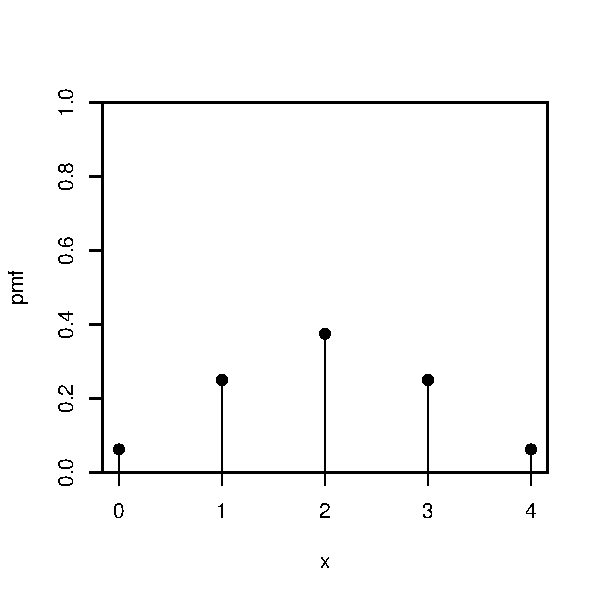
\includegraphics[width=1.5in]{figures/Binpmf.pdf}
  \end{minipage}
  The PMF satisfies
  \[p_X(x) \geq 0 \textrm{ and } \sum_x p_X(x) = 1 \]
  
	\item[Parameter:]  a quantity that can be assigned any one of a number of possible values, with each different value determining a different probability distribution in $p_X(x;\alpha)$
	\item[Family of probability distributions:] The collection of all probability distributions for different values of the parameter\\
	\vspace{2pt}
Example of a family of distributions for a \emph{bernoulli random variable}, $X$, with $O_x = \left \{ {0, 1} \right \}$
\begin{align*}
& \text{parameter for } P(X=1) = \alpha = p_X(x;\alpha)\\
& \text{parameter for } P(X=0) = 1-\alpha = p_X(x;\alpha)\\
& \text{family of distributions for } p_X(x;\alpha) = \left\{\begin{array}{lcl} 1-\alpha &; & \mbox{x=0}; \\ \alpha; &; & \mbox{x=1}; \\ 0 & ; & \mbox{otherwise} \end{array} \right.
\end{align*}
%%% CDF
	\item[Cumulative Distribution Function (cdf)]: The cdf $F$ of a d.r.v. $X$ with probability mass function $p_X$ is described by
\[F_X(x)=P(X \leq x)=\sum_{y \in O_x : y \leq x}{p_X(y)} \text{ (the sum of probability masses)}\]
For any number $x$, $F_X(x)$ is the probability that the observed value of $X$ will be at most $x$.
\begin{minipage}{\linewidth}
            \centering
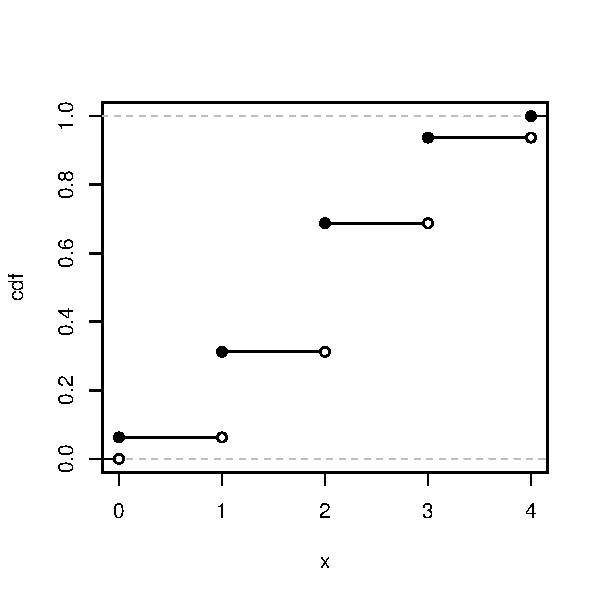
\includegraphics[width=1.5in]{figures/Bincdf.pdf}
        \end{minipage}
The CDF is an increasing, right-continuous function with  \begin{center}
$F_X(x) \to 0 \textrm{ as $x \to -\infty$ and } F_X(x) \to 1 \textrm{ as $x \to \infty$}$
\end{center}

\item[Independence] Two random variables are independent if knowing the value of one gives no information about the other. Discrete r.v.s $X$ and $Y$ are independent if for \emph{all} values of $x$ and $y$  \begin{center}
$P(X=x, Y=y) = P(X = x)P(Y = y)$
\end{center}
\end{description}

\subsection{Expectation}
\begin{description}

\item[Expected Value] (a.k.a.~\emph{mean}, \emph{expectation}, or \emph{average}) is a weighted average of the possible outcomes of our random variables. Mathematically, if $x_1, x_2, x_3, \dots$ are all of the distinct possible values that $X$ can take, the expected value of $X$ is
\begin{center}
$E(X) = \mu_X = \sum\limits_{i}x_iP(X=x_i) = \sum\limits_{i}x_ip_X(x_i)$
\end{center}

\begin{minipage}{\linewidth}
            \centering
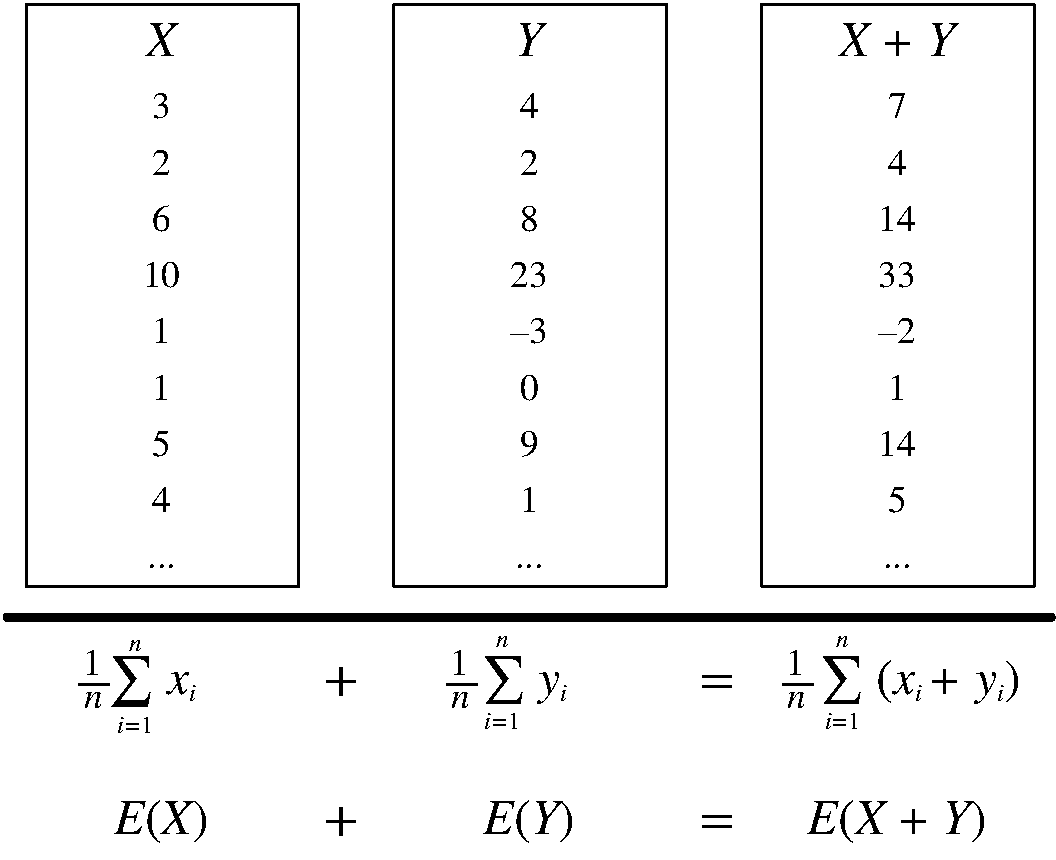
\includegraphics[width=2in]{figures/linearity.pdf}
        \end{minipage}
        
\item[Functions of Random Variables] Let $X$ be a d.r.v with pmf $p$ and let $g$ be a function from the real numbers to the real numbers, $g:\mathbb{R} \rightarrow \mathbb{R}$. The function $g$ on $X$, $g(X)$, is also a r.v. with pmf $p(x)$
\begin{center}
$E[g(x)]=\sum g(x) P[g(X)=x] = \sum_{x} g(x)p(x)$
\end{center}
In addition, it can be shown that
\begin{center}
$E[g(x)]=g[E(X)]$
\end{center}
\item[Linearity] For any r.v.s $X$ and $Y$, and constants $a,b,c,$ 
\[E(aX + bY + c) = aE(X) + bE(Y) + c \]
Short proof: Let $g(X) = aX + b$
\begin{center}
$E[g(X)] = \sum_{x \in O_x} (ax+b)p(x) = \sum_x axp(x) + bp(x)$
$= a\sum xp(x) + b\sum p(x) = aE(X)+b = g[E(X)]$
\end{center}
\item[Uniform Random Variables] For r.v. $X$ where all outcomes have the same probability, $p(x_i)=p(x_j) \forall i,j \in k$
\begin{center}$E(X) = \frac{1}{k}{\sum_j x_j} = \frac{k+1}{2}$\end{center}

\item[Bernoulli Random Variables] For a Bernoulli r.v. $X$ having binary outcomes, where $\alpha$ is the probability $X=1$ and $1-\alpha$ is the probability $X=0$,
\begin{center}
$p(x;\alpha) = \left\{\begin{array}{lcl} 1-\alpha &; & \mbox{x=0}; \\ \alpha; &; & \mbox{x=1}; \\ 0 & ; & \mbox{otherwise} \end{array} \right.$
\end{center}
\begin{center}$E(X) = \sum\limits_{x \in {0, 1}}x\cdot p(x) = 0 \cdot (1 - \alpha) + 1 \cdot \alpha = \alpha$\end{center}

\item[Geometric Random Variables] Let $X$ be geometric r.v. for the number of babies born until the first girl, where $G$ is the event the baby is a girl, $P(G_i) = g \forall i$
\begin{align*}
& f(1)=P(G_1)=g \\
& f(2)=P(!G_1 \cap G_2)=(1-g) \cdot g \\
& f(3)=(1-g)^2 \cdot g \\
& f(x;g)== \left\{\begin{array}{lcl} (1-g)^{x-1} \cdot g &; & x \in \left \{1, 2, \dots \right \}; \\ 0 & ; & \mbox{otherwise} \end{array} \right.
\end{align*}

\begin{center}
$E(X) = \sum\limits_{x \in \left \{ {1, 2 \dots } \right \}}x \cdot (1-g)^{x-1} \cdot g = \frac{1}{g}$
\end{center}

\item[Same distribution implies same mean] If $X$ and $Y$ have the same distribution, then $E(X)=E(Y)$ and, more generally, 
$$E(g(X)) = E(g(Y))$$

\item[Conditional Expected Value] is defined like expectation, only conditioned on any event $A$. \begin{center}
$\ E(X | A) = \sum\limits_{x}xP(X=x | A)$
\end{center}

\item[Variance and Standard Deviation] Let $X$ be a random variable and let $\mu=E(X)$.\\
\vspace{3pt}
The variance of $X$ is defined as $var(X)=E[(X-\mu)^2]$\\
The standard deviation of $X$ is defined as $\sigma_x=\sqrt{var(x)}$
  \begin{align*}
    var(X) & = E[X^2-2X\mu+\mu^2] = E(x^2)-E(2X\mu)+E(\mu^2) \\
    & = E(X^2)-2\mu E(X)+\mu^2 = E(X^2)-2\mu^2+\mu^2 \\
    & = E(X^2)-\mu^2=E(X^2)-[E(X)]^2
  \end{align*}
  Properties \\
  \quad Let $c\in\mathbb{R}$.
  \begin{enumerate}
    \item $var(X+c)=E[(X+c-E(X+c))^2] = E[(X+c-E(X)-c)^2]= var(X)$
    \item$var(cX)=E[(cX-E(cX)^2]=E[(cX-cE(X))^2]=E[c^2(X-E(ZX))^2]=c^2E[(x-E(x))^2]=c^2var(X)$
  \end{enumerate}
\end{description}

%%% Distributions

\subsection{Discrete Distributions}
\subsubsection{Binomial Probability Distribution}
\begin{description}
  \item[Binomial Experiment] is defined by the following characteristics:
  \begin{enumerate}
    \item The experiment consists of a sequence of $n$ smaller experiments called \emph{trials}, where $n$ is fixed in advance of the experiment.
    \item Each trial can result in one of the same two possible outcomes (dichotomous trials), which we generically denote by success (S) and failure (F).
    \item The trials are independent, so that the outcome on any particular trial does not influence the outcome on any other trial.
    \item The probability of success P(S) is constant from trial to trial; we denote this probability by $p$.
  \end{enumerate}
  \item[Rule] Consider sampling without replacement from a dichotomous population of size $N$. If the sample size (number of trials) $n$ is at most 5\% of the population size, the experiment can be analyzed as though it were exactly a binomial experiment.
  \item[Binomial Random Variable] A binomial r.v. $X$ associated with a binomial experiment consisting of $n$ trials with success probability $p$ is defined as
  \[X \sim Bin(n, p)\]
  \item[pmf of a Binomial r.v.] Because the pmf of a binomial rv $X$ depends on the two parameters $n$ and $p$, the pmf is denoted by $b(x; n, p)$.
    \begin{center}
       $b(x; n, p) = \left\{\begin{array}{{lcl}} \left(^n_x \right)p^x(1-p)^{n-x} &; & x= 0, 1, 2, \dots, n  \\ 0 &; & otherwise \end{array} \right.$
    \end{center}
  \item[cdf of a Binomial r.v.] For $X \sim Bin(n, p)$, the cdf is denoted by
    \begin{center}
      $B(x; n, p) = P(X \leq x) = \sum_{y=0}^x b( y; n, p) \quad x = 0, 1, \dots , n$
    \end{center}
  \item[Mean, Variance and SD of Binomial r.v.] If $X \sim Bin(n, p)\text{, then }$
    \begin{center}
      $E(X) = np\text{, }V(X)=np(1-p) = npq \text{, and }$ \\
      $\sigma_x =  \sqrt{npq}\text{ ( where }q = 1 - p)$
    \end{center}
\end{description}

%%%%%%%%%%%%%%%%%%%%%%%%%%%%%%%%%%%%%%%%%%%%%%%%%%%%%%%%%%%%%%%%
% Unit 4.2: Continuous Random Variables
%%%%%%%%%%%%%%%%%%%%%%%%%%%%%%%%%%%%%%%%%%%%%%%%%%%%%%%%%%%%%%%%
\section{Unit 4.2 Continous Random Variables}
	\subsection{Terms and Definitions}
\begin{description}
	\item[Continuous Set:] is a set of connected points with a continuous interval
	\item[Continuous Random Variable (c.r.v.):] is a function whose domain is the sample space $\mathscr{S}$ and whose range is a continuous interval or set of intervals of real numbers in the probability space $(\mathscr{S}, \mathscr{F}, P)$, , but the probability of any one value is zero.
      \[X:\mathscr{S} \rightarrow \mathbb{R}\]
      \[X(\omega) = 0\]
%%% PDF
	\item[Probability Density Function (pdf):] The pdf $f$ of a c.r.v. $X$ in the problem space $(\mathscr{S}, \mathscr{F}, P)$ is described by 
    \[P(a \leq X \leq b) = \int_{x=a}^b{f(x)dx}\]
	\item[Cumulative Distribution Function (cdf):] The cdf $F(x)$ for a c.r.v $X$, is the area under $f$ from $-\infty$ to $x$:
	\begin{center}
	$F(x)=P(X \leq x) = \int_{y=-\infty}^x{f(y)dy}$
	\end{center}
Properties
    \begin{enumerate}
    \item The derivative of the cdf $F$ is the pdf $f$
    \begin{center}
    $F'(x) = f(x)$
    \end{center}
    \item A pdf is nonnegative and integrates to $1$. 
    \begin{center}
    $\int_{y=-\infty}^\infty{f(y)dy} = 1$
    \end{center}
    \item By the fundamental theorem of calculus, we can integrate pdf to get back to cdf:
    \begin{center} 
        $F(x) =\int_{-\infty}^x f(t)dt$
       \end{center}
       \begin{minipage}{\linewidth}
                \centering
    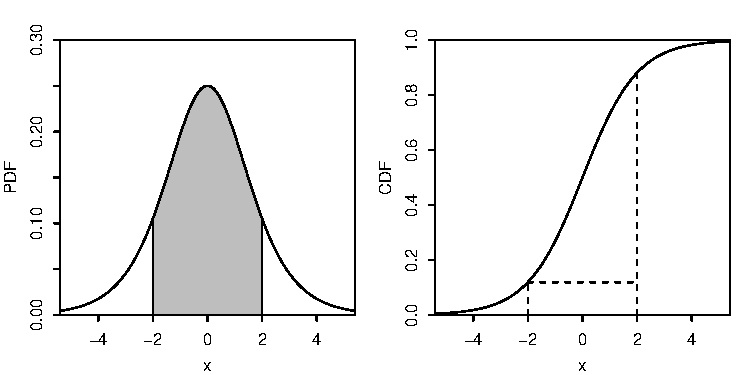
\includegraphics[width=2in]{figures/Logisticpdfcdf.pdf}
            \end{minipage}
       To find the probability that a c.r.v. takes on a value in an interval, integrate the pdf over that interval.
          \begin{center} 
        $F(b) - F(a) =  \int^b_a f(x)dx$
           \end{center}
    \end{enumerate}
\end{description}

\subsection{Expectation}
\begin{description}
  \item[Expected value of an r.v.]
  The expected value of $X$ is defined as:
  \[E(X) = \sum_x xP(X=x) \textnormal{ (for discrete $X$)}\]
  
  \item[Expected value of a function of an r.v.] A function of a r.v. is also a r.v. If $h:\mathbb{R}\rightarrow \mathbb{R}$  then $h(x)$ is a random variable and \\
  $$E(h(x))=\int_{x=-\infty}^\infty h(x)f(x)dx$$
  
The \textbf{Law of the Unconscious Statistician (LOTUS)} states that you can find the expected value of a \emph{function of a random variable}, $g(X)$, in a similar way, by replacing the $x$ in front of the PMF/PDF by $g(x)$ but still working with the PMF/PDF of $X$:
\[E(g(X)) = \sum_x g(x)P(X=x) \textnormal{ (for discrete $X$)}\]
\[E(g(X)) = \int^\infty_{-\infty}g(x)f(x)dx \textnormal{ (for continuous $X$)}\]
Properties
  \begin{enumerate}
    \item if $h(x) = aX+b$  then $E(h(x)) = aE(X)+b$
  \end{enumerate}
  
  \item[Variance and Standard Deviation] 
   Let X have pmf $p(x)$ and expected value $\mu$.  Then the $ V(X)$ or $\sigma_{X}^2$ is
  $$V(X) = \sum_{D}(x-\mu)^2 \cdot p(x) = E[(X-\mu)^2]$$
  The standard deviation (SD) of X is $\sigma = \sqrt{\sigma}$\\
  Alternatively,
  $$ V(X) = \sigma^2 = \big[\sum_{D}x^2 \cdot p(x)\big] - \mu^2 = E(X^2) - [E(X)]^2$$
  Properties
  \begin{enumerate}
  	\item $V(aX + b) = a^2 \cdot \sigma^2$
  	\item In particular, $\sigma_{aX} = |a| \cdot \sigma_{x}$
  	\item $\sigma_{X+b} = \sigma_{X}$
  \end{enumerate}
\end{description}

\subsection{Continuous Distributions}
\subsubsection{Uniform Distribution}
\begin{description}
  \item[pdf of Uniform Random Variable] $X$ has a uniform distribution on $[A,B]$ if it has probably density function\\
  \begin{center}
  $f(x)=\left\{\begin{array}{lcl} \frac{1}{B-A} &; & A \leq x \leq B \\ 0 & ; & \mbox{otherwise} \end{array} \right.$
  \end{center}


When $X$ is between $A$ and $B$,\\
$$F(x)=\int_{-\infty}^{x}f(y)dy = \int_{A}^{x}\frac{1}{B-A}dy={\frac{y}{B-A}} \bigg\rvert_{a}^{x}=\frac{x-A}{B-A}$$
\begin{center}
$F(x) = \left\{\begin{array}{lcl} 0 &; & \mbox{x<A}; \\ \frac{x-A}{B-A}; &; & {A \leq x \leq B}; \\ 1 & ; & B \leq x \end{array} \right.$
\end{center}


\begin{minipage}{\linewidth}
  \centering
  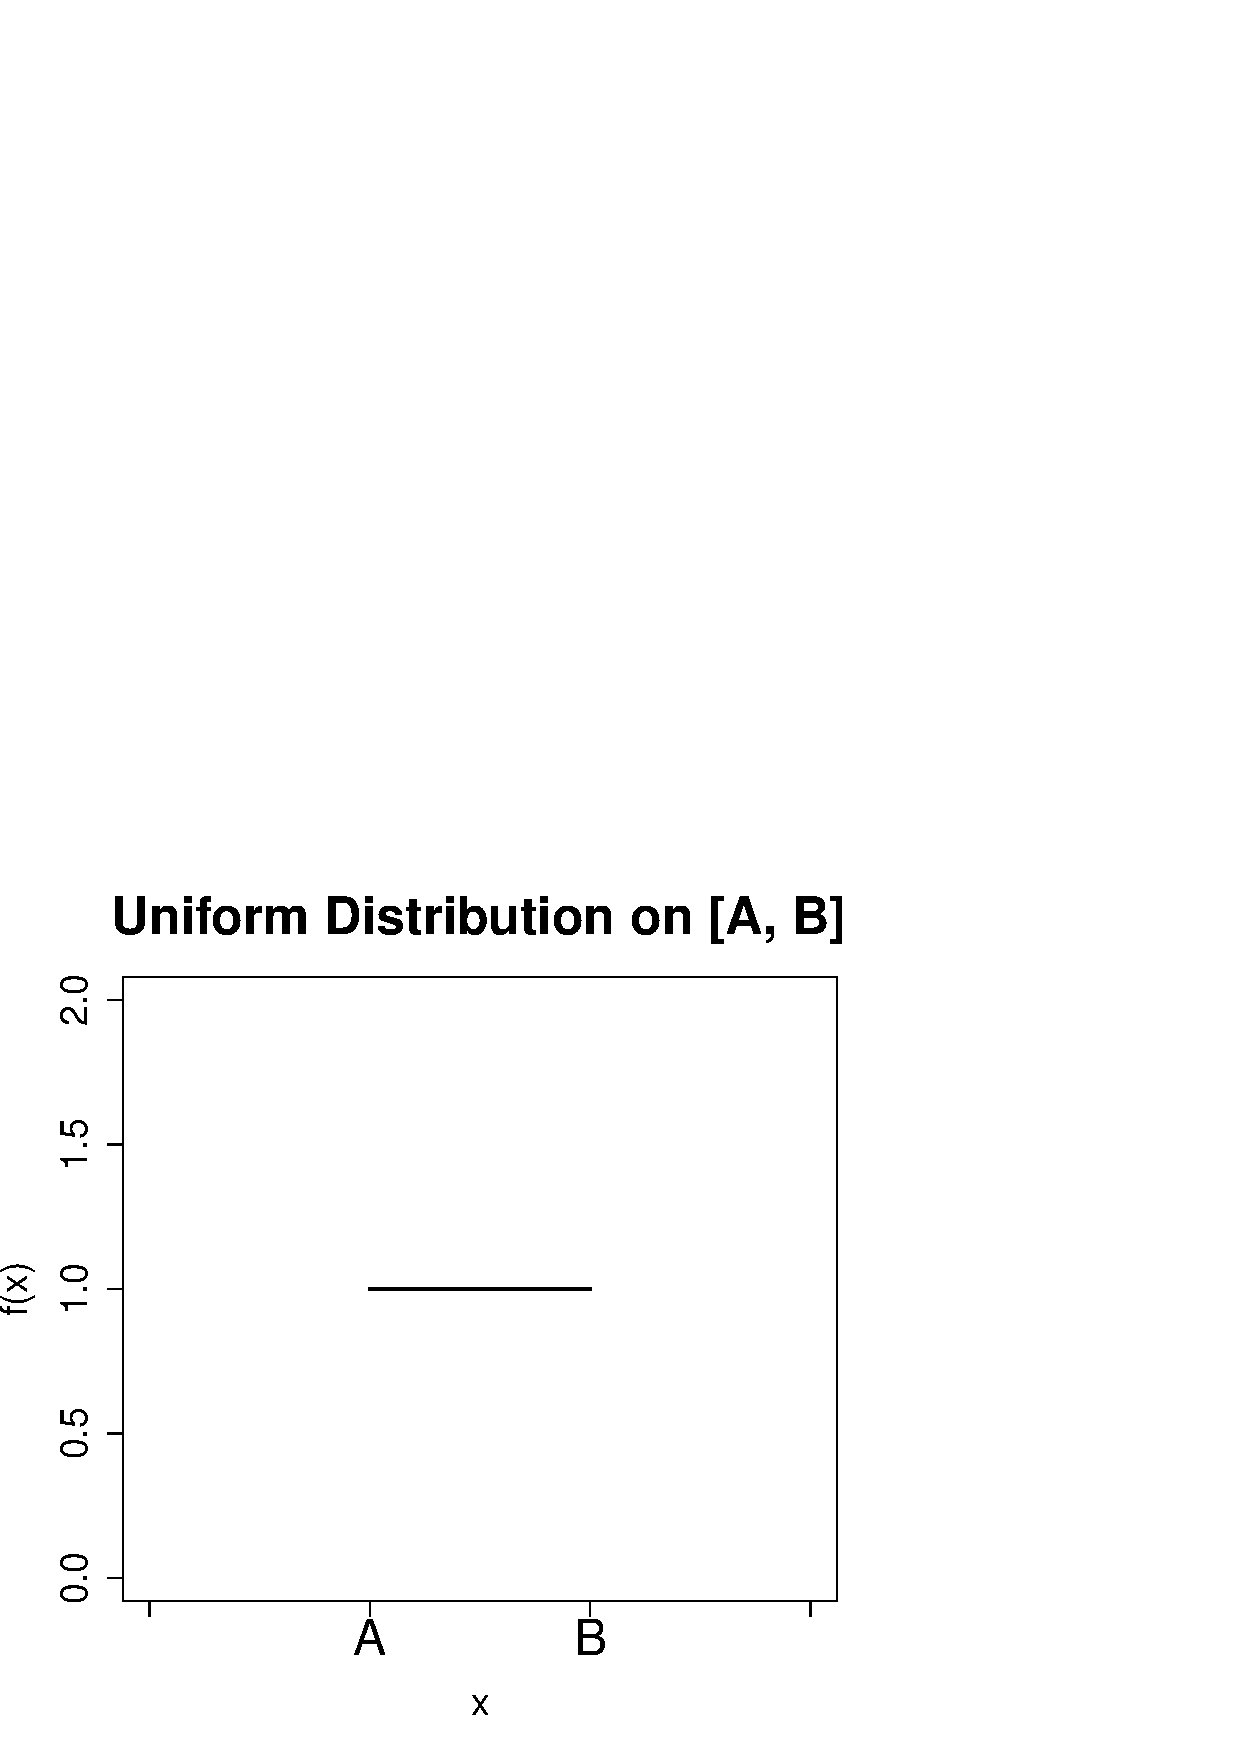
\includegraphics[width=3cm]{W203_Unit_Summary-uniform_pmf}
  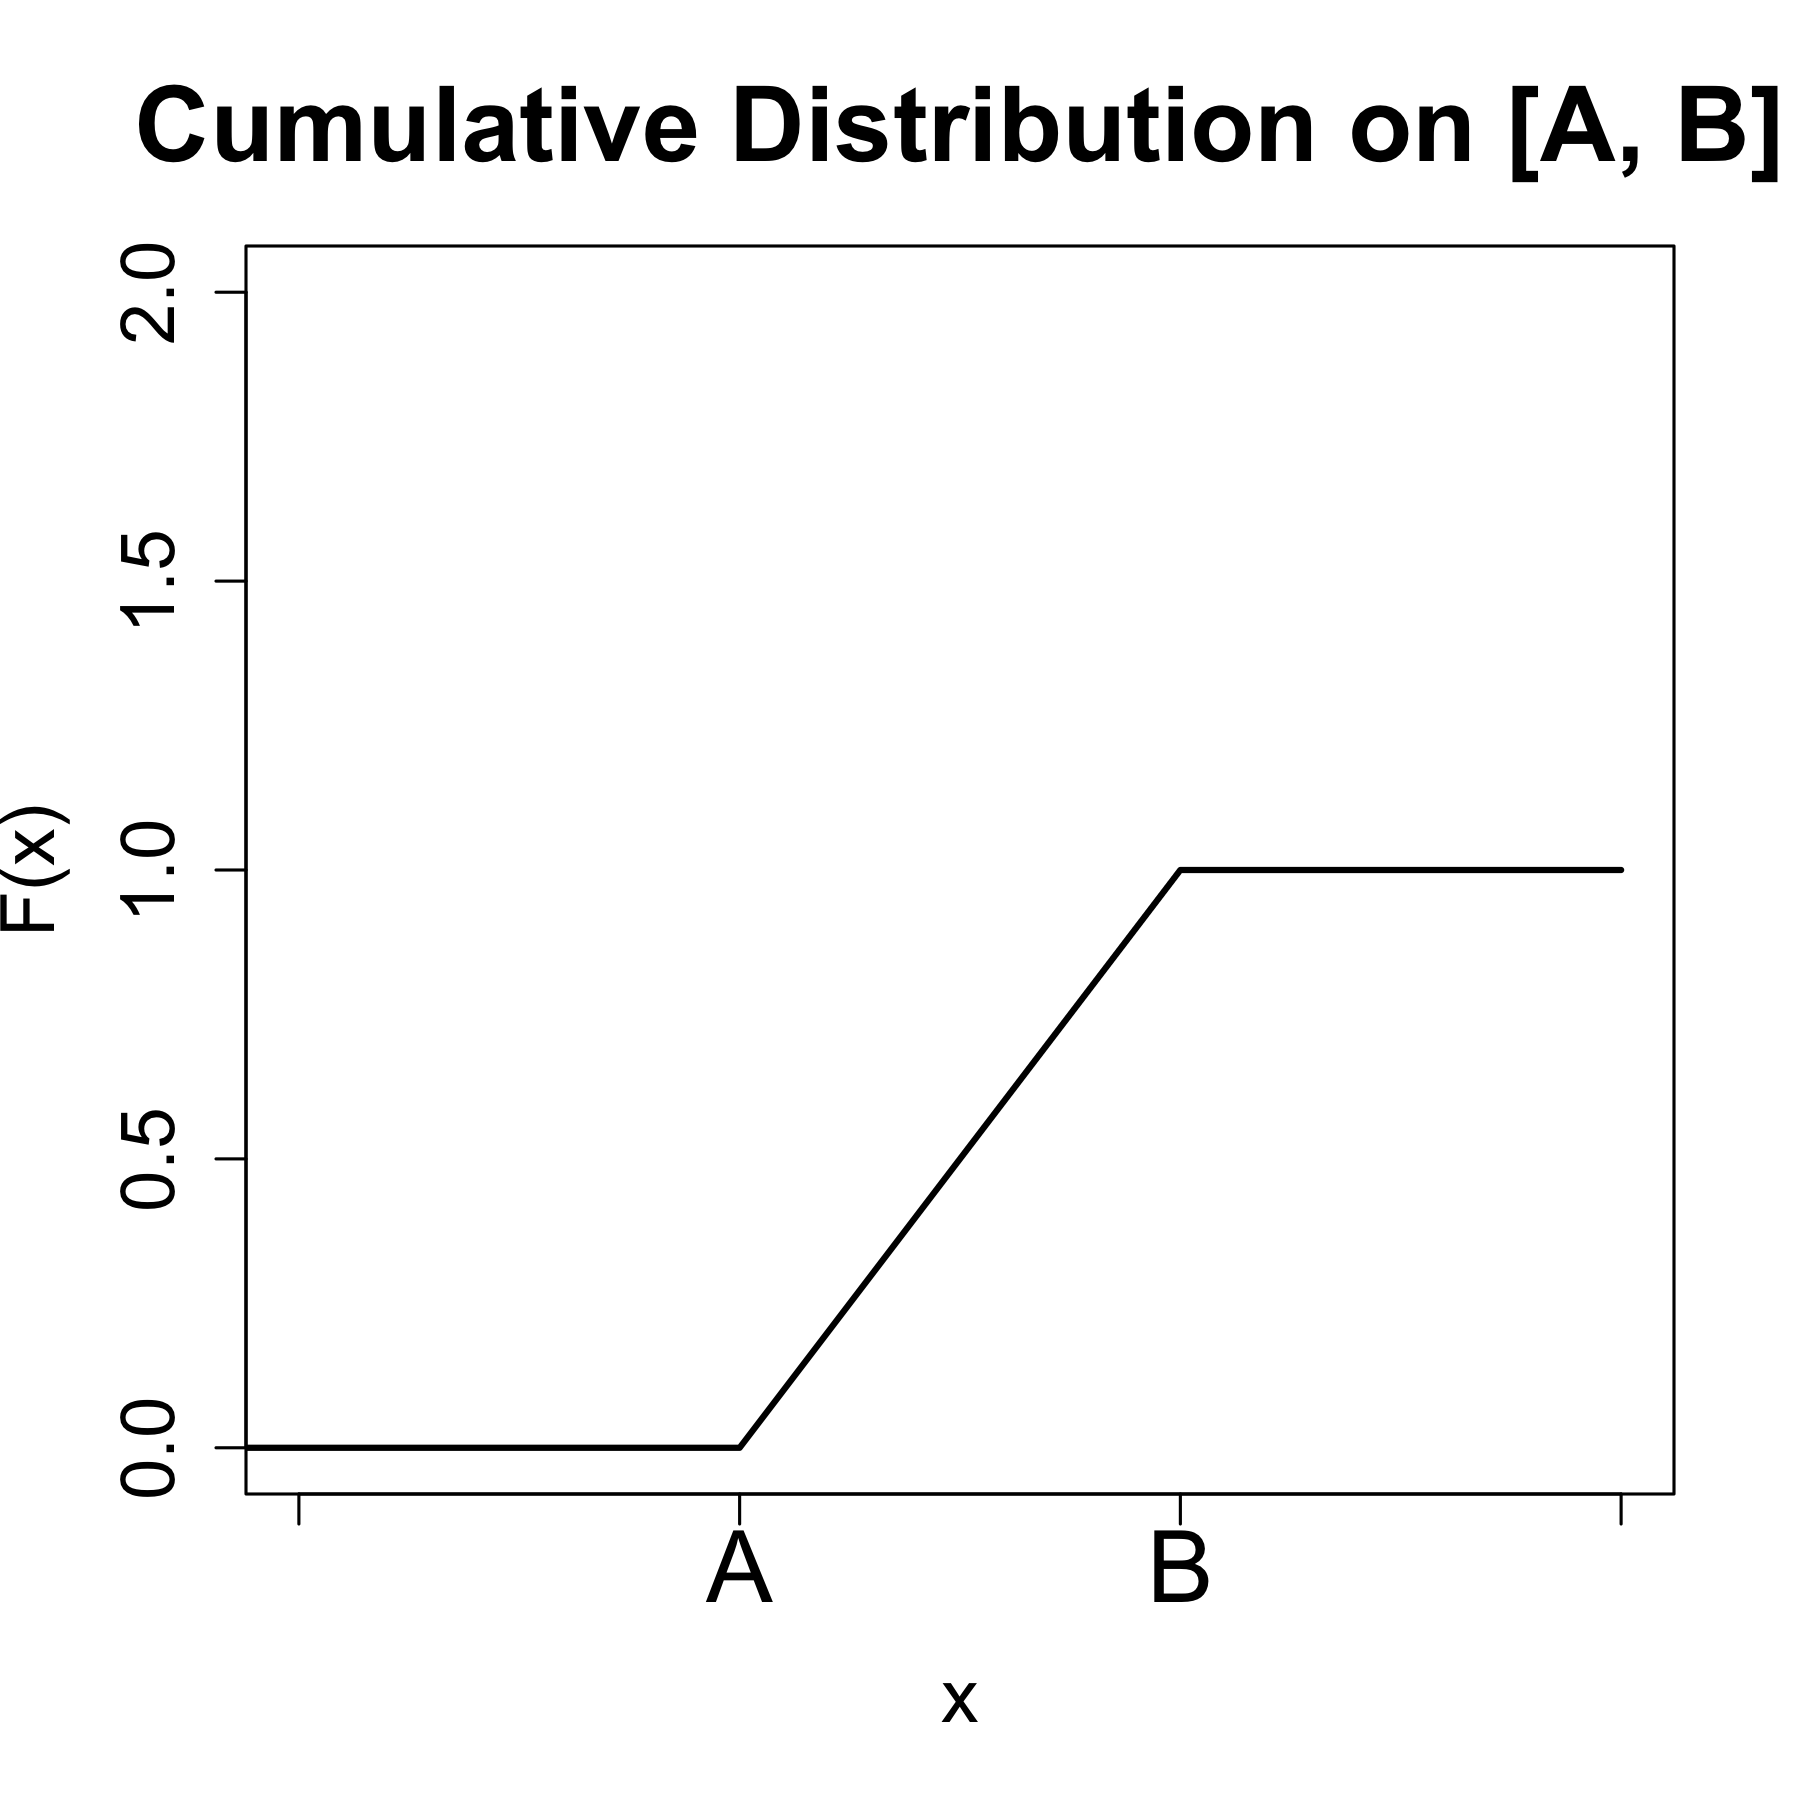
\includegraphics[width=3cm]{W203_Unit_Summary-uniform_cdf}
\end{minipage}


\item[Expectation] \quad
\begin{center}
$E(X) = \int_{-\infty}^{\infty}x \cdot f(x)dx = \int_{A}^{B}x \cdot \frac{1}{B-A}dx$ \\
$= \frac{x^2}{2\cdot(B-A)}\bigg\rvert_{A}^{B}=\frac{B^2-A^2}{2 \cdot(B-A)} = \frac{A+B}{2}$
\end{center}
\item[Variance] \quad
\begin{center}
$Var(X) = E(X^2) - [E([X)]^2$
\end{center}
\begin{center}
$[E([X)]^2 = \int_{-\infty}^{\infty}x^2 \cdot f(x)dx = \int_{A}^{B}x^2 \cdot \frac{1}{B-A}dx$ \\
$= \frac{x^3}{3\cdot(B-A)}\bigg\rvert_{A}^{B}=\frac{B^3-A^3}{3 \cdot(B-A)} = \frac{A^2+2AB+B^2}{3}$
\end{center}
\begin{center}
$Var(X) = \frac{A^2+2AB+B^2}{3} - (\frac{A+B}{2})^2 = \frac{A^2+2AB+B^2}{3} - \frac{A^2+2AB+B^2}{4}$
$= \frac{A^2-2AB+B^2}{12} = \frac{(B-A)^2}{12}$
\end{center}
\end{description}

\subsubsection{Normal Distribution}
\begin{description}
   \item[Normal Distribution Random Variable] The statement that X is normally distributed with parameters $\mu$ and $\sigma^2$ is often abbreviated $X \sim N(\mu,\sigma^2).$
  \item[pdf of a Normal Distribution r.v.] A c.r.v $X$ is said to have a normal distribution with parameters $\mu$ and $\sigma$ (or $\mu$ and $\sigma^2$), where $-\infty < \mu < \infty$ and $0 < \sigma$ when the pdf of $X$ is:
  \begin{center}
  $f(x; \mu, \sigma) = \frac{1}{\sqrt{2\pi\sigma^2}}e^{-(x-\mu)^2/2\sigma^2} -\infty < x < \infty$
  \end{center}
  Properties
  \begin{enumerate}
    \item $\mu$, the location parameter, is both the mean and the median.
    \item $\sigma$, the scale parameter, stretches the curve horizontally.
  \end{enumerate}
  \item[Mean, Variance and SD of a Normal Distribution r.v.] It can be shown that $E(X) = \mu$ and $V(X) = \sigma^2$, so the parameters are the mean and the standard deviation of X.\\
  Properties
  \begin{enumerate}
    \item 68\% of the area is within 1 standard deviation of the mean.
    \item 95\% of the area is within 2 standard deviations of the mean.
    \item 99.7\% of the area is within 3 standard deviations of the mean.
  \end{enumerate}

  \item[Standard Normal Distribution] defined as Z, or $\phi(z)$, is when $\mu=0$ and $\sigma=1$
  \begin{center}
    $\text{pdf}:  \quad \phi(z) = \frac{1}{\sqrt{2 \pi}} e^{-z^{2}/2} \qquad \text{cdf}: \quad  \Phi(z) = \int_{-\infty}^{z} \phi(u) du$
  \end{center}
  \item[Standardizing a Normal Variable] is when we take a normal variable that is not standard normal, and adjust it. The new random variable becomes $\frac{(X-\mu)}{\sigma}$, and we can express probabilities involving X in terms of the z-distribution.
  \item[Deviations from Normality] \quad \\
  Skewness
  \begin{enumerate}
    \item Negative Skew - tail is to the left
    \item Positive Skew - tail is to the right
  \end{enumerate}
  Kurtosis
  \begin{enumerate}
    \item Platykurtic - flatter and smooshed down
    \item Leptokurtic - much more bunched together and peek up.
  \end{enumerate}
  
\end{description}

%%%%%%%%%%%%%%%%%%%%%%%%%%%%%%%%%%%%%%%%%%%%%%%%%%%%%%%%%%%%%%%%
% Unit 5: Joint Distributions
%%%%%%%%%%%%%%%%%%%%%%%%%%%%%%%%%%%%%%%%%%%%%%%%%%%%%%%%%%%%%%%%
\section{Unit 5: Joint Distributions}
	\subsection{Terms and Definitions}
\begin{description}
  \item[Joint Range:] Let $X:\mathcal{S} \to \mathbb{D}_1$ and $Y:\mathcal{S} \to \mathbb{D}_2$ be 2 rvs with a common sample space. We define the joint range of the vector $(X,Y)$ of the form
$$  \mathbb{D} = \mathbb{D}_1 \times \mathbb{D}_2 = \{ (x,y): x \in \mathbb{D}_1, y \in \mathbb{D}_2\} $$

  \item[Random Vector:] A 2-D random vector$(X,Y)$ is a function from $\mathcal{S} \to \mathbb{R}^2$.  It is defined $\forall \omega \in \mathcal{S}$ such that $$ (X,Y)(\omega) = (X(\omega), Y(\omega)) = (x,y) \in \mathbb{D}$$
  
  \item[Joint Probability Distribution or Joint Probability Mass Function:] For two d.r.v.'s $X$ and $Y$.  The joint pmf of $(X,Y)$ is defined $\forall (x,y) \in \mathbb{D}$
$$  p(x_{i}, y_{j}) = P(X = x_{i}, Y = y_{j}) $$
It must be that $p(x,y) \geq 0$ and $\sum_i \sum_j p(x_{i}, y_{j}) = 1$.
  \item[Marginal Prob Mass Function:] of $X$ and of $Y$, denoted $p_{X}(x)$ and $p_{Y}(y)$ respectively,
$$  p_{X}(x) = \sum_{y: p(x,y) >0} p(x,y) \quad \forall x \in \mathbb{D}_1$$

	\item[Joint Probability Density Function:] For two c.r.v.'s $X$ and $Y$.  The joint pdf of $(X,Y)$ is defined $\forall A \subseteq \mathbb{R}^2$
$$  P((X,Y)\in A) = \iint_{A} f(x,y)dx dy $$
It must be that $f(x,y) \geq 0$ and $\int_{-\infty}^{\infty} \int_{-\infty}^{\infty} f(x, y) dx dy= 1$. Note also that this integration is commutative.

  \item[Marginal Prob Density Function:] of $X$ and of $Y$, denoted $f_{X}(x)$ and $f_{Y}(y)$ respectively,
$$  f_{X}(x) = \int_{-\infty}^{\infty} f(x,y) dy \quad \forall x \in \mathbb{D}_1$$

Note that if $f(x,y)$ is the joint density of the random vector $(X,Y)$ and $A \in \mathbb{R}^2$ is of the form $A= [a,b]\times[c,d]$ we have that
$$  P((X,Y)\in A) = \int_{c}^{d} \int_{a}^{b} f(x, y) dx dy = \int_{a}^{b} \int_{c}^{d} f(x, y) dx dy $$

  \item[Independence:] Two rvs are independent if 
$$ P(X=x, Y=y) = P(X=x) P(Y=y) \quad  f(x,y) = f_{X}(x) f_{Y}(y)$$

  \item[Conditional Distribution(discrete):] For two discrete rv's $X$ and $Y$ with joint pmf $p(x_{i}, y_{j})$ and marginal $X$ pmf $  p_{X}(x)$, then for any realized value $x$ in the range of $X$, the conditional mass function of $Y$, given that $X=x$ is 
$$  p_{Y|X}(y|x) = \frac{p(x_{i}, y_{j})}{p_{X}(x)} $$

  \item[Conditional Distribution(continuous):] For two continuous rv's $X$ and $Y$ with joint pdf $f(x,y)$ and marginal $X$ pdf $  f_{X}(x)$, then for any realized value $x$ in the range of $X$, the conditional density function of $Y$, given that $X=x$ is 
$$  f_{Y|X}(y|x) = \frac{f(x, y)}{f_{X}(x)} $$

\subsection{Expected Values, Covariance \& Correlation}

\item[Expected value:] The expected value of a function $h(X, Y)$ of two jointly distributed r.v.'s is  
\[E(h(X, Y)) = \sum_x\sum_yh(x, y)P(X=x, Y=y) \text{ for discrete r.v.}\] 
\[E(h(X, Y)) = \int_{-\infty}^{\infty}\int_{-\infty}^{\infty}h(x, y)f_{X,Y}(x, y)dxdy \text{ for continuous r.v.}\]

\item[Covariance:] Measures the strength of the relation btwn 2 RVs, however very 
$$ Cov(X,Y) = E[(X-E(X))(Y - E(Y))] = E(XY) - E(X)E(Y) $$
Shortcut Formula:
$$	Cov(X,Y) = E(XY)  -  \mu_{x} \mu_{y}$$

The defect of the covariance however is that its value depends critically on the units of measurement.

\item[Correlation:] Cov after standardization. Helps interpret Cov. 
$$ \rho =  \rho_{X,Y} = Corr(X,Y) = \frac{Cov(X,Y)}{\sqrt{V(X)V(Y)}} = \frac{Cov(X,Y)}{SD(X) SD(Y)} $$
Has the property that $Corr(aX+b, cY+d) = Corr(X,Y)$\\
and that for any rvs X, Y $-1 \leq \rho \leq 1$.\\

Note also that $\rho$  is independent of units, the larger $|\rho|$ the stronger the linear association, considered strong linear relationship if $|\rho| \geq 0.8$.\\

Caution though: if X and Y are independent then $\rho = 0$ but $\rho =0$ does not imply that X,Y are independent.\\
Also that $\rho = 1$ or $-1$ iff $Y = aX+b$ for some $a,b$ with $a\neq0$.
\end{description}


%%%%%%%%%%%%%%%%%%%%%%%%%%%%%%%%%%%%%%%%%%%%%%%%%%%%%%%%%%%%%%%%
% Unit 6: Sampling and the Central Limit Theorem
%%%%%%%%%%%%%%%%%%%%%%%%%%%%%%%%%%%%%%%%%%%%%%%%%%%%%%%%%%%%%%%%
\section{Unit 6: Sampling and the Central Limit Theorem}
	\subsection{Terms and Definitions}
\begin{description}

\item[Statistic:] Any quantity whose value can be calculated with sample data. Prior to obtaining data, there is uncertainty as to what value of any particular statistic will result. Therefore, a statistic is a random variable and will be denoted by an uppercase letter; a lowercase letter is used to represent the calculated or observed value of the statistic.\\
\item[Sampling Distribution:] The probability distribution of a statistic. It describes how the statistic varies in value across all samples that might be selected and how much uncertainty we have in our statistics\\
\begin{enumerate}
  \item If the sampling distribution is wide, we could get very different values each time we draw a new sample, so we have little confidence in the numbers we get.
  \item If the sampling distribution is narrow, we would get similar values each time we repeat the experiment.\\
      We only get one number, but we believe that it's representative (i.e., more meaningful).
  \item A centerpiece of statistics is estimating how much uncertainty exists within the statistics collected.\\
      Distinguishes statistics from other fields like machine learning
\end{enumerate}
\item[Unit of analysis:] the singular unit that defines all the different cases in a given study.
\item[Population:] the entire set of all units of analysis, every single one.\\
\item[Selected Sample:] is who we target and who we try to reach.\\
\item[Actual Sample:] is who responds.\\
\item[Sampling Design:] our specific strategy for obtaining a sample, which is presumably going to be representative of the larger population. Examples include quota sampling, random sampling, snowball sampling, stratified random sampling, and convenient sampling.
\item[Problems with Sampling Design:] 1) getting a representative sample 2) one or two outliers skewing the data 3) controlling bias in the sampling method
\item[Important issue in samples:] All other things being equal, a small simple random sample of 100 people is preferable to a convenience sample of 10,000 people from the same population. A small random sample will give better estimates of the population despite the smaller sample size.\\
\item[Examples of Bias:] 1) Non-voters who do not respond. 2) Those who acre the most are more likely to respond 3) Interviewer inconsistencies in selecting who to interview 4) Self-selection sampling - waiting for people to decide whether to take it versus recruiting people randomly

The point here is that we need to anticipate bias. We need to find it even when we didn't anticipate it, and we need to deal with it. So it's always better, always better to acknowledge potential bias, rather than to assume it does not exist at all

\item[The chance error:] is the stuff that we expect. That's the stuff that we know is part of just doing statistics. We can at least estimate how much error that is, how much chance error there is.

Statistic (what we know) = parameter(what we want to know) + bias + chance error.

Try to use procedures that take biases out of the equation

\item[Sampling Frame:] A list of units of analysis from which you take a sample: Directories, Local census, Registered users of an online system\\
\item[Simple Random Samples] The researcher has no discretion over who is included. The procedure for selecting a sample is definite; it involves planned use of chance.
\item[Simple Random Sample: Procedure] \quad
\begin{enumerate}
  \item Requires numbering all potential participants in a given sampling frame (N)
  \item Pulls random numbers from any source and uses the random numbers to create the sample (n)
  \item Has an equal chance of each value being selected
  \item Issues:\\
  1) True randomization (seeding random number generators)\\
  2) Replacement in the field (e.g., door-to-door problem)\\
\end{enumerate}
\item[Stratified Random Sampling:] \quad
\begin{enumerate}
  \item Key issue: representation of salient subpopulations\\
    Maximizes between-group variance while minimizing within-group variance
  \item For proportionate samples:\\
  1) Do you know the key independent variables?\\
  2) If not, you may be better off avoiding stratification\\
  \item For disproportionate samples:\\
    Sample weighting is used because some groups are much smaller or larger than others.\\
  \item Example - Obtaining a sample of participants: \\
  1) We will attempt to obtain an equal number of survey participants (100 maximum per strata) from five different editing strata.\\
  2) We oversample those who edit more because they make up a smaller percentage of the population.\\
\end{enumerate}
\item[Cluster Sampling:] \quad
\begin{enumerate}
  \item Randomly selected clusters are specifically sampled from
  \item Used when there are no available sampling frames
  \item Based on areas, institutions, or “clusters”
\end{enumerate}
\item[Respondent-Driven Sampling:] \quad
\begin{enumerate}
  \item Combines snowball sampling with a mathematical model that weights the sample
  \item Compensates for the nonrandom collection of the sample
\end{enumerate}

\item[Non-probability Sampling:] \quad
\begin{enumerate}
  \item Quotas  \quad \\
   1) Pick key groups of interest and find individuals to fill specific goals.\\
   2) Quotas are fulfilled without using random sampling.\\
  \item Purposive sampling  Find key groups and only study them.
  \item Convenience sampling  Taking anyone you can get to participate
  \item Snowball sampling  Finding a starting point and using these individuals to get next participant
\end{enumerate}


\item[Survey Weight:] is a numeric value that is assigned to each case in our dataset.
\item[Weighted Value:] indicates how much each case (each unit of analysis) will count in any type of statistical analysis or procedure that is run.

\item[Types of Weights:] \quad
\begin{enumerate}
  \item Design weights
  \begin{enumerate}
    \item Used to correct for oversampling or undersampling specific cases\\
        Example: Smaller groups in the population may be oversampled, such as Linux users compared to PC and Mac users.
    \item Correct proper representation in the population
  \end{enumerate}
  \item Poststratification weights
  \begin{enumerate}
    \item Used to correct for the fact that some types of cases are less likely to show up in the sample\\
      Example: People of different age groups differ in how likely they are to respond to surveys.
    \item Used to correct for actual proportions in the population
  \end{enumerate}
\end{enumerate}

\item[Weighting With Multiple Characteristics] \quad
\begin{enumerate}
  \item Weight the sample by the first characteristic.
  \item Then generate the frequency for the second characteristic from this weighted data.
  \item Calculate the second characteristic weight.
  \item Generate a final weight by multiplying the two weights.
\end{enumerate}

\item[Random Sampling:] The rv's $X_1, X_2, \cdots X_n$ are said to form a (simple) random sample of size n if
\begin{enumerate}
  \item The Xi's are independent rv's.
  \item Every Xi has the same probability distribution.
  \item Think of this as an ideal case.\\
      Real-world sampling may deviate from this, but we usually try to get as close to random sampling as we can.
  \item We can often rephrase this by saying the Xi's are independent and identically distributed (iid).
  \item If we sample randomly from a population with replacement, we satisfy the conditions for random sampling.
  \item  If we sample from an infinite population (a generating process that gives us as independent number of independent draws), we also have random sampling.
  \item Random sampling is approximately satisfied if sampling is without replacement, yet the sample size n is much smaller than the population size N, and each unit of observation has the same probability of being sampled. \\
  In practice, as long as we draw 5\% of the population or less, and each unit of observation has the same probability of being sampled, we usually proceed as though we have a random sample.
\end{enumerate}
\item[The Distribution of the Sample Mean: ] Let $X_1, X_2, \cdots, X_n$ be independent and identically distributed random variables with mean $\mu$ and deviation $\sigma$. Then
\begin{enumerate}
  \item $E(\bar{X})=\mu_{\bar{X}}=\mu$
  \item $Var(\bar{X})=\sigma_{\bar{X}}^2=\frac{\sigma^2}{n}$
  \item $\sigma_{\bar{X}} = \sqrt{Var(\bar{X})} = \frac{\sigma}{\sqrt{n}}$
\end{enumerate}

\item[Central Limit Theorem:] Let $X_1, X_2, \cdots, X_n$ be a random sample from a distribution with mean $\mu$ and variance $\sigma^2$. Then if $n$ is sufficiently large, $\bar{X}$ has approximately a normal distribution with $\mu_{\bar{X}}$ and $\sigma_{\bar{X}}^2 = \frac{\sigma^2}{n}$. The larger the value of $n$, the better the approximation. When to apply:
  \begin{enumerate}
    \item The degree to which the population distribution is non-normal determines whether to use the CLT.
    \item A common rule of thumb in statistics says to use the CLT if n > 30.
    \item 30 is enough for the vast majority of distributions you'll encounter.
    \item It's still worth looking at your data before applying the CLT.
    \item If you have a very unusual distribution \\
        E.g., something extremely skewed \\
        E.g., it can take n = 100, or perhaps even n = 1000 to achieve a normal distribution\\
    \item Very unusual distributions are rare.
  \end{enumerate}

\end{description}

\end{multicols}
\end{document}
